\documentclass{article}
\usepackage{graphicx}
\usepackage[T1]{fontenc}
\usepackage[utf8]{inputenc}
\usepackage[polish]{babel}
\usepackage{amsmath}

\title{Sprawozdanie laboratorium lista 2 - obliczenia naukowe}
\author{\normalsize Zofia Tarchalska}
\date{}

\begin{document}
\maketitle


\section{Zadanie 1}
Celem zadania było powtórzenie zadania 5 z listy 1, ale z lekko zmodyfikowanymi danymi. Dokładnie chodziło o to aby usunąć ostatnią 9 z czwartej współrzędnej wektora x i ostatnią 7 z piątej współrzędnej. Wektory te prezentują się następująco:\\
\noindent $x = [2.718281828, -3.141592654, 1.414213562, 0.5772156649, 0.3010299957]$\\
\noindent $y = [1486.2497, 878366.9879, -22.37492, 4773714.647, 0.000185049]$\\

\noindent Po zmianie:\\
$x = [2.718281828, -3.141592654, 1.414213562, 0.577215664, 0.301029995]$\\

\noindent Po lewej: poprzednie uzyskane wyniki. Po prawej: nowe wyniki\\

\noindent
\begin{minipage}{0.48\textwidth}
\begin{verbatim}
Float32
real: -1.00657107000000e-11
forward: -0.4999443
backward: -0.4543457
biggest_to_smallest: -0.5
smallest_to_biggest: -0.5

Float64
real: -1.00657107000000e-11
forward: 1.0251881368296672e-10
backward: -1.5643308870494366e-10
biggest_to_smallest: 0.0
smallest_to_biggest: 0.0
\end{verbatim}
\end{minipage}
\hfill
\begin{minipage}{0.48\textwidth}
\begin{verbatim}
Float32
-----------------------------
forward: -0.4999443
backward: -0.4543457
biggest_to_smallest: -0.5
smallest_to_biggest: -0.5

Float64
-----------------------------
forward: -0.004296342739891585
backward: -0.004296342998713953
biggest_to_smallest: -0.004296342842280865
smallest_to_biggest: -0.004296342842280865
\end{verbatim}
\end{minipage}

\noindent \\\\Można zauważyć, że jeśli chodzi o arytmetykę single wyniki w ogóle nie różnią się od tych uzyskanych w poprzedniej próbie. Dzieje się tak, ponieważ usuwane cyfry są na gracnicy precyzji. Inaczej jest w przypadku double, w tej arytmetyce otrzymujemy różne rezultaty. 

\subsection*{Wnioski} Okazuje się, że w przypadku arytmetyki Float64 niewielka zmiana na 10 miejscu po przecinku powoduje zmianę wyniku o 7 rzędów wielkości. Najpierw wynik był rzędu $10^{-10}$ żeby następnie wzrosnąć rzędu $10_{-3}$ (dla sposobu forawrd i backward, ponieważ są to te bardziej precyzyjne sposoby). Widzimy zatem, że zadanie jest źle uwraunkowane (mała zmiana w danych powoduje duże zmiany wyniku).

\section{Zadanie 2}
W zadaniu należy narysować wykres funkcji $f(x) = e^xln(1+e^{-x})$ w co najmniej dwóch różnych programach do wizualizacji. Następnie trzeba policzyć jej granicę i porównać z otrzymanymi wykresami.\\
\noindent
\begin{minipage}{0.48\textwidth}
    \begin{center}
        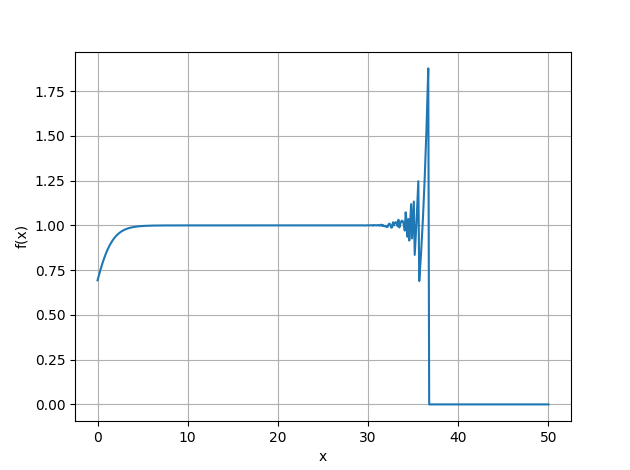
\includegraphics[width=1\textwidth]{pyplot_fx.png}
    \end{center}
\end{minipage}
\hfill
\begin{minipage}{0.48\textwidth}
    \begin{center}
        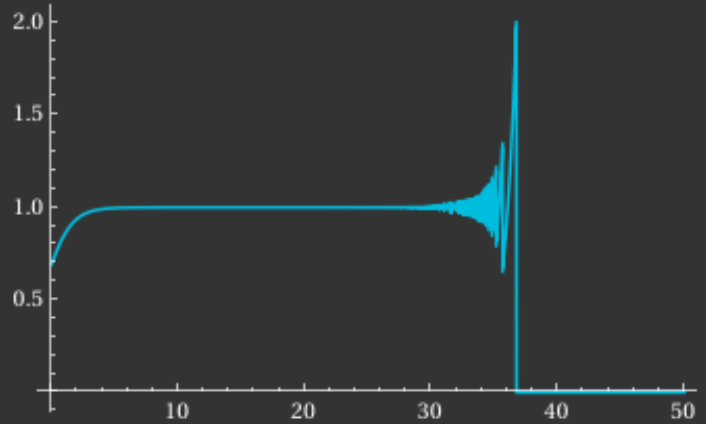
\includegraphics[width=1\textwidth]{wolfram_fx.png}
    \end{center}
\end{minipage}

\noindent Po lewej widnieje wykres wygenerowany za pomocą PyPlot, a po prawej w WolframAlpha.

\noindent Teraz ręcznie policzmy granicę funkcji w nieskończoności:
\[
 \lim_{x \to \infty } e^x \cdot ln(1 + e^{-x}) = \lim_{x \to \infty} \frac {-e^{-x}}{(1 + e^{-x}) \cdot (-e ^{-x})} = \lim_{x \to \infty} \frac{1}{1 + e^{-x}} = 1
\]

\noindent Jak widać rzeczywisty przebieg funckji różni się od tego co zwracają nam obydwa programy.
\subsection*{Wnioski} 
Znów zadanie charakteryzuje się silnym uwarunkowaniem numerycznym. Niedokładności wynikające z ograniczonej percyzji, prowadzą do odchyleń wartości funkcji od prawidłowego wyniku, szczególnie w zakresie $x \in [30, 36]$. Dla argumentów $>36$ funkcja zbiega do 0, ponieważ zachodzi przybliżenie $ 1 + e^{-x} \approx 1$ zatem $ln(1 + e^{-x}) \approx 0$. Jest to sprzeczne z rzeczywistym przebiegiem funkcji i wyznaczoną granicą analityczną. Zaburzenie występuje w obydwu programach zewnętrznych, co oznacza złe uwarunkowanie zadania.

\section{Zadanie 3}
Zadanie polegało na rozwiązaniu układu równań liniowych dwoma różnymi sposobami oraz porównaniu ich pod kątem policzonych błędów względnych.


\noindent \\ Mamy równanie liniowe postaci: $Ax = b$, gdzie: \\
\begin{itemize}
\item A to macierz współczynników. Generujemy ją na dwa sposoby:\\
    \begin{itemize}
        \item $A = H_n$, gdzie $H_n$ jest macierzą Hilberta stopnia n 
        \item $A = R_n$, gdzie $R_n$ to losowa macierz stopnia n z podanym wskaźnikiem uwarunkowania c
    \end{itemize}
\item b to wektor prawych stron
\end{itemize}

\noindent Układ ten będziemy rozwiązywać dwoma metodami:
\begin{itemize}
    \item metodą eliminacji Gauss'a - $x = A \backslash b$
    \item metodą z macierza odwrotną - $x = inv(A) * b$
\end{itemize}

\noindent Nasz dokładny $x$ to $x = (1, ..., 1)^T$. Z jego pomocą będziemy obliczać błąd względny. Na nastęnych stronach zamieszczone zostają wartości zwracane przez funkcje \texttt{rank(A)} i \texttt{cond(A)} oraz policzone błędy względne dla obu metod.
\newpage
\begin{verbatim}
Macierz Hilberta

n   cond(A)                  rank(A) error Gauss              error inv
1   1.0                      1       0.0                      0.0
2   19.28147006790397        2       5.661048867003676e-16    1.4043333874306803e-15   
3   524.0567775860644        3       8.022593772267726e-15    0.0
4   15513.73873892924        4       4.137409622430382e-14    0.0
5   476607.2502422687        5       1.6828426299227195e-12   3.3544360584359632e-12   
6   1.49510586424659e7       6       2.618913302311624e-10    2.0163759404347654e-10   
7   4.753673565921816e8      7       1.2606867224171548e-8    4.713280397232037e-9
8   1.5257575538072489e10    8       6.124089555723088e-8     3.07748390309622e-7
9   4.931537556012197e11     9       3.8751634185032475e-6    4.541268303176643e-6
10  1.602441350036382e13     10      8.67039023709691e-5      0.0002501493411824886
11  5.222703245009594e14     10      0.00015827808158590435   0.007618304284315809
12  1.760619121841585e16     11      0.13396208372085344      0.258994120804705
13  3.1905581877988255e18    11      0.11039701117868264      5.331275639426837
14  9.27636978936766e17      11      1.4554087127659643       8.71499275104814
15  3.67568286586649e17      12      4.696668350857427        7.344641453111494
16  7.063115212292111e17     12      54.15518954564602        29.84884207073541
17  8.07124989431416e17      12      13.707236683836307       10.516942378369349
18  1.4135073701749765e18    12      10.257619124632317       24.762070989128866
19  5.190132496359103e18     13      102.15983486270827       109.94550732878284
20  1.3193976166344822e18    13      108.31777346206205       114.34403152557572
21  3.2903033202156175e18    13      44.089455838364245       34.52041154914292
22  8.482350008309597e18     13      17.003425713362045       102.60161611995359
23  6.101209031674573e17     13      25.842511917947366       22.272314298730727
24  1.8162451419244399e19    13      39.638573210187644       43.34914763015038
25  1.3309197553221074e18    13      7.095757204652332        21.04404299195525
26  7.779515179373411e18     14      63.80426636186403        100.78434642499187       
27  4.28683702161786e18      14      27.43309009053957        35.68974530952139
28  5.937872779302876e18     14      276.91498822022265       290.1167291705239
29  8.277434084408434e18     14      60.095450394724104       43.40383683199056
30  3.8719824664564173e18    14      24.80615905441871        59.97231132227779
31  9.796434738176467e18     14      21.45662601984968        23.74575780277118
32  4.2803982785172644e18    14      36.582441571177284       67.4381226943068
33  1.1705168465593727e19    14      37.556822732776205       32.88969741379979
34  5.546235957952042e18     14      88.87380459381126        95.99116506490785
35  2.552419613144824e19     14      31.166902974731222       36.723963451169304
36  4.227992561870757e18     15      15.563379312608328       19.599011323097056
37  5.859007350289631e18     15      13.974714130452178       16.39248770656996
38  8.652991891691735e18     15      72.12122789133323        95.5655782183542
39  1.8383449979886094e19    15      118.2033650158989        263.5309838641091
40  6.581732387647914e18     15      23.926484807638683       140.97274594056717
41  1.5426903357896567e19    15      41.348771577098454       40.75749340255354
42  2.9056333619025285e19    15      229.6423260398746        333.75226335487844
43  1.4838416581923312e19    15      53.18930954995267        54.52704305417691
44  2.6895334840373182e19    15      124.67413636996756       94.88356401052424
45  1.214705872715781e19     15      244.58124814685374       179.92316617880468
46  1.5097027936171698e19    15      69.14584939886464        109.17112219679052
47  1.9943467382012723e20    15      41.43803149349301        83.82203728470039
48  1.0925283248003965e19    15      58.952689545073156       156.78973560359313
49  6.093374357739825e18     16      24.150620097509638       35.92139018094681
50  1.0993264246156683e19    16      63.36958239742337        69.99768122728986
\end{verbatim}
\begin{verbatim}
Macierz losowa

n   c                        rank(A) error Gauss              error inv
5   1.000000000000001        5       1.4043333874306804e-16   2.2752801345137457e-16   
5   9.999999999999996        5       2.482534153247273e-16    2.432376777795247e-16
5   1000.0000000000236       5       2.9790409838967276e-16   4.203627514058621e-15
5   9.999999998130372e6      5       5.799015982916193e-11    1.377444663806729e-10
5   9.999322361505425e11     5       8.767946479620035e-6     1.101328684658636e-5
5   4.3389446864305475e15    4       0.5593130377167642       0.5591916598984644
10  1.000000000000001        10      5.15985034193911e-16     3.3121136700345433e-16
10  9.999999999999993        10      2.8737410463596867e-16   2.4575834280036907e-16
10  999.9999999999911        10      2.293995889930822e-14    2.7609708695270473e-14
10  9.999999990916912e6      10      2.0955792024649492e-10   1.81840723377465e-10
10  9.99976991136977e11      10      4.196755515487614e-5     3.614790502971321e-5
10  1.7803773341590864e16    9       0.14037179426228394      0.13931683203224224
20  1.0000000000000016       20      5.382005793715205e-16    3.9409007944299576e-16
20  10.0                     20      7.854386543748146e-16    6.309740391678007e-16
20  1000.0000000000028       20      3.120208680502288e-14    3.6192861929420846e-14   
20  9.99999999564815e6       20      1.603342362471366e-10    1.5697362145029217e-10
20  1.0000134366492958e12    20      1.6168699871775732e-5    1.4716047607150038e-5
20  8.563256185085127e15     19      0.3290975485091718       0.32066957992953976
\end{verbatim}

\subsection*{Wnioski}
\noindent Możemy zauważyć, że macierze Hilberta osiągają bardzo duże wartości współczynnika uwarunkowania (parametr \texttt{cond(A)}) już przy stosunkowo niewielkich rozmiarach n. Wysoki wskaźnik uwarunkowania oznacza, że układ $Ax = b$ jest źle uwarunkowany, czyli nawet niewielkie błędy w danych (w macierzy A lub w b) mogą prowadzić do dużych błędów w rozwiązaniu.Eksperymenty pokazują, że możemy to zaobserowować zarówno dla metody eliminacji Gauss'a jak i metody z użyciem odwrotności macierzy. Oznacza to, że numeryczne rozwiązanie układu Hilberta jest trudne do uzyskania z dużą dokładnością.\\
Dla losowych macierzy z ustalonym współczynnikiem uwarunkowania
c, błędy względne są małe i podobne dla obu metod. Oznacza to, że algorytmy są stabilne numerycznie dla macierzy dobrze uwarunkowanych.


\end{document}